%\documentclass[a4,semhelv,landscape]{seminar}
\documentclass[landscape]{slides}
%\documentclass[pdf, default, slideBW, nocolorBG]{prosper}
\usepackage[left=0.2cm,top=0.2cm,right=0.2cm,bottom=0.2cm,nohead,nofoot]{geometry}
%\def\everyslide{\sffamily}
%\usepackage{fullpage}
\usepackage{graphicx}
\usepackage[usenames]{color}
%\usepackage{color}
\usepackage{verbatim}
\usepackage{nopageno}
\usepackage{setspace}
%\usepackage{times}
% define some nice colors
\definecolor{myred}{rgb}{0.6,0,0}
\definecolor{myblue}{rgb}{0,0.2,0.4}
\definecolor{mygreen}{rgb}{0,0.5,0.0}
\definecolor{mypurple}{cmyk}{0.5,1.0,0.0,0.0}
\definecolor{myorange}{cmyk}{0.0,0.75,1.0,0.0}
%\color{myblue}

\begin{document}
%%%%%%%%%%%%%%%%%%%%%%%%%%%%%%%%%%%%%%%%%%%%%%%%%%%%%%%%%%%%%%%%%%%%
%Slide 0 - title
\begin{slide}
\begin{center}
\large{\textbf{Reference-guided annotation of viral genomes}}

\normalsize

Eric Nawrocki \\

\medskip

\medskip

\medskip

\medskip

\medskip

\small
\begin{tabular}{c}
%Alejandro Sch\"{a}ffer's group \\
%\\
National Center for Biotechnology Information\\
National Institutes of Health\\
\\
\end{tabular}

\vspace{0.1in}

\includegraphics[width=2.5in]{figs/ncbi-logo}

\end{center}
\end{slide}
%%%%%%%%%%%%%%%%%%%%%%%%%%%%%%%%%%%%%%%%%%%%%%%%%%%%%%%%%%%%%%%%%%%%%%
\begin{slide}
\begin{center}

\textbf{Most prevalent viral genomes in GenBank\footnote{Current as of March, 2018.}}

\tiny
\begin{tabular}{r|l|r|l|l|l|r|r}
     &                     &              &                &          &        &       & \#mature \\ 
rank & species             & \#seqs       & family         & type     & host   &  \#CDS& peptides \\ \hline
     &                     &              &                &          &        &       &          \\ 
  1  &  Influenza          &   503,115    & Orthomyxoviridae& (-)ssRNA& humans+&    11 & -        \\ %NC_007370
     &                     &              &                &          &        &       &          \\ 
  2  & Rotavirus A         &58,405\footnote{sum of 11 segments}& Reoviridae&dsRNA&humans&   12 & -\\ %NC_011503
     &                     &              &                &          &        &       &          \\ 
  3  & Hepatitis B         &         9211 & Hepadnaviridae & dsDNA-RT & humans &     7 & -        \\ %NC_003977
     &                     &              &                &          &        &       &          \\ 
  4  & Dengue              &         4853 & Flaviviridae   & (+)ssRNA & humans &     1 & 14       \\ %NC_001477
     &                     &              &                &          &        &       &          \\ 
  5  & HIV-1               &        2597  & Retroviridae   & ssRNA-RT & humans &    10 & 14       \\ %NC_001802
     &                     &              &                &          &        &       &          \\ 
  6  & Hepatitis C         &        2185  & Flaviviridae   & (+)ssRNA & humans &     2 & 10       \\ %NC_004102
     &                     &              &                &          &        &       &          \\ 
  7  & Porcine circovirus  &        1905  & Circoviridae   & ssDNA    & pigs   &     3 & -        \\ %NC_005148
     &                     &              &                &          &        &       &          \\ 
  8  & West Nile           &        1667  & Flaviviridae   & (+)ssRNA & humans &     3 & 16       \\ %NC_009942
     &                     &              &                &          &        &       &          \\ 
  9  & Ebola               &        1384  & Flaviviridae   & (+)ssRNA & humans &     9 & -        \\ %NC_002549
     &                     &              &                &          &        &       &          \\ 
 10  & Enterovirus A       &        1222  & Picarnoviridae & (+)ssRNA & humans &     1 & 11       \\ %NC_001612
     &                     &              &                &          &        &       &          \\ 
 11  & RSV                 &        1122  & Orthopneumovirus& (-)ssRNA& humans &    11 & -        \\ %NC_001781
     &                     &              &                &          &        &       &          \\ 
 12  & Norwalk virus       &        1009  & Calciviridae   & (+)ssRNA & humans &     3 & 6        \\ %NC_029646
     &                     &              &                &          &        &       &          \\ 
 13  & Maize streak virus  &         884  & Geminiviridae  & ssDNA    & plants &     4 & -        \\ %NC_001346
     &                     &              &                &          &        &       &          \\ 
 14  & Rabies lyssavirus   &         826  & Rhabdoviridae  & (-)ssRNA & humans+&     5 & -        \\ %NC_001542
     &                     &              &                &          &        &       &          \\ 
 15  & Enterovirus C       &         765  & Picarnoviridae & (+)ssRNA & humans &     1 & 13       \\ %NC_002058
\end{tabular}

\tiny
\flushright{$\dagger$ sum of 11 segments}
\vfill

\end{center}
\end{slide}
%%%%%%%%%%%%%%%%%%%%%%%%%%%%%%%%%%%%%%%%%%%%%%%%%%%%%%%%%%%%%%%%%%%%%%
\end{document}
o%%%%%%%%%%%%%%%%%%%%%%%%%%%%%%%%%%%%%%%%%%%%%%%%%%%%%%%%%%%%%%%%%%%%%%
\begin{slide}
\begin{center}
\textbf{The Virus Variation Resource is a powerful tool for viral research}

\begin{minipage}[c]{4in}
\tiny
\begin{itemize}
\item value added database that includes annotations not in GenBank
\item allows users to: 
\begin{itemize}
  \item select subsets of data based on desired criteria
    (host, country, gene, etc.)
  \item download alignments
  \item  compute trees
  \item  more...
\end{itemize}
\end{itemize}
\vfill
\end{minipage}
\begin{minipage}[c]{6in}
\includegraphics[width=6in]{figs/viv-page1}
\vfill
\end{minipage}

\vfill
\end{center}
\end{slide}
%%%%%%%%%%%%%%%%%%%%%%%%%%%%%%%%%%%%%%%%%%%%%%%%%%%%%%%%%%%%%%%%%%%%%%
\begin{slide}
\begin{center}
\textbf{The Virus Variation Resource is a powerful tool for viral research}

\includegraphics[width=8.5in]{figs/viv-dengue-query}

\vfill
\end{center}
\end{slide}
%%%%%%%%%%%%%%%%%%%%%%%%%%%%%%%%%%%%%%%%%%%%%%%%%%%%%%%%%%%%%%%%%%%%%%
\begin{slide}
\begin{center}
\textbf{Our goal is to develop an annotation pipeline to benefit \\ Virus Variation}

\small
\begin{itemize}
\item general method for annotating existing and new viral genome
  sequences for a species using trusted annotation for that species (e.g. RefSeq)
\item identify interesting characteristics that Virus Variation can
  allow users to sort/select based on:
\begin{itemize}
  \item identification of high quality sequences that meet specific expectations
  \item identification of sequences that deviate from expectations in
    various ways
    \begin{itemize}
      \item early stop codon
      \item above or below a specific fractional identity to reference 
      \item more...
    \end{itemize}
\end{itemize}
\end{itemize}

\end{center}
\vfill
\end{slide}
%%%%%%%%%%%%%%%%%%%%%%%%%%%%%%%%%%%%%%%%%%%%%%%%%%%%%%%%%%%%%%%%%%%%%%
\begin{slide}
\begin{center}
\textbf{Outline of talk}

\small
\begin{description}
\item[1.] Selection of four pilot viral species
\item[2.] Overview of annotation pipeline and explanation of ``error codes''
\item[3.] Statistics on pilot phase annotations
\item[4.] Implementation of annotation pipeline
\item[5.] Interaction with J. Rodney Brister's Virus Variation group
\item[6.] Future directions
\end{description}

\end{center}
\vfill
\end{slide}

%%%%%%%%%%%%%%%%%%%%%%%%%%%%%%%%%%%%%%%%%%%%%%%%%%%%%%%%%%%%%%%%%%%%%%
\begin{slide}
\begin{center}
\textbf{Outline of talk}

\small
\begin{description}
\item[\textcolor{myorange}1.] \textcolor{myorange}{Selection of four pilot viral species}
\item[2.] Overview of annotation pipeline and explanation of ``error codes''
\item[3.] Statistics on pilot phase annotations
\item[4.] Implementation of annotation pipeline
\item[5.] Interaction with J. Rodney Brister's Virus Variation group
\item[6.] Future directions
\end{description}

\end{center}
\vfill
\end{slide}

%%%%%%%%%%%%%%%%%%%%%%%%%%%%%%%%%%%%%%%%%%%%%%%%%%%%%%%%%%%%%%%%%%%%%%
\begin{slide}
\begin{center}

\textbf{Four pilot species were chosen from the 15 most prevalent}

\tiny
\begin{tabular}{r|l|r|l|l|l|r|r}
       &                    &              &                &          &        &       & \#mature \\ 
  rank & species            &       \#seqs & family         & type     & host   & \#cds & peptides \\ \hline
       &                    &              &                &          &        &       &          \\ 
\textcolor{myorange}{1} & \textcolor{myorange}{Hepatitis B}        &         \textcolor{myorange}{7061} & \textcolor{myorange}{Hepadnaviridae} & \textcolor{myorange}{dsDNA-RT} & \textcolor{myorange}{humans} &     \textcolor{myorange}{7} &       \textcolor{myorange}{-}  \\
       &                    &              &                &          &        &       &          \\ 
\textcolor{myorange}{2} & \textcolor{myorange}{Dengue}             &         \textcolor{myorange}{3875} & \textcolor{myorange}{Flaviviridae}   & \textcolor{myorange}{(+)ssRNA} & \textcolor{myorange}{humans} &     \textcolor{myorange}{1} &      \textcolor{myorange}{14}  \\
       &                    &              &                &          &        &       &          \\ 
     3 & Rotavirus          &      22536*  & Reoviridae     & dsRNA    & humans &    12 &       -  \\
       &                    &              &                &          &        &       &          \\ 
     4 & HIV-1              &        2132  & Retroviridae   & ssRNA-RT & humans &    10 &      14  \\
       &                    &              &                &          &        &       &          \\ 
     5 & Porcine circovirus &        1559  & Circoviridae   & ssDNA    & pigs   &     3 &       -  \\
       &                    &              &                &          &        &       &          \\ 
     \textcolor{myorange}{6} & \textcolor{myorange}{West Nile}          &        \textcolor{myorange}{1109} & \textcolor{myorange}{Flaviviridae}   & \textcolor{myorange}{(+)ssRNA} & \textcolor{myorange}{humans} &     \textcolor{myorange}{3} &      \textcolor{myorange}{16}  \\
       &                    &              &                &          &        &       &          \\ 
     7 & Hepatitis C        &        1457  & Flaviviridae   & (+)ssRNA & humans &     2 &      10  \\
       &                    &              &                &          &        &       &          \\ 
     8 & Ebola              &        1105  & Flaviviridae   & (+)ssRNA & humans &     9 &       -  \\
       &                    &              &                &          &        &       &          \\ 
     9 & Enterovirus A      &         932  & Picarnoviridae & (+)ssRNA & humans &     1 &      11  \\
       &                    &              &                &          &        &       &          \\ 
    10 & RSV                &         623  & Paramyxoviridae& (-)ssRNA & humans &    11 &       -  \\
       &                    &              &                &          &        &       &          \\ 
    11 & Enterovirus C (Polio) &      618  & Picarnoviridae & (+)ssRNA & humans &     1 &      13  \\
       &                    &              &                &          &        &       &          \\ 
    12 & JC polyomavirus    &          598 & Polyomaviridae & dsDNA    & humans &     6 &       -  \\
       &                    &              &                &          &        &       &          \\ 
    13 & PRRSV              &          520 & Arteriviridae  & (+)ssRNA & pigs   &    11 &      13  \\ %# 15 mat_peptide segments, 13 mat_peptides 
       &                    &              &                &          &        &       &          \\ 
    \textcolor{myorange}{14} & \textcolor{myorange}{Maize streak virus} &          \textcolor{myorange}{508} & \textcolor{myorange}{Geminiviridae}  & \textcolor{myorange}{ssDNA}    & \textcolor{myorange}{plants} &     \textcolor{myorange}{4} &      \textcolor{myorange}{-}   \\
       &                    &              &                &          &        &       &          \\ 
    15 & Norwalk virus      &          491 &  Calciviridae  & (+)ssRNA & humans &     3 &       6  \\ 
\end{tabular}

\end{center}

\tiny
\flushright{$*$ sum of 11 segments}
\vfill
\end{slide}
%%%%%%%%%%%%%%%%%%%%%%%%%%%%%%%%%%%%%%%%%%%%%%%%%%%%%%%%%%%%%%%%%%%%%%
\begin{slide}
\begin{center}
\textbf{Maize Streak Virus}

\begin{minipage}[c]{6in}
\tiny
\begin{itemize}
\item cause of most serious crop disease in Africa, responsible for
  between USD\$100-\$500 million of crop loss per year
\item NC\_001346 (2689 nt):
  \begin{itemize}
    \item 4 CDS (V1, V2, C1, C1:C2), 5 total ‘exons’
    \item both strands have $>=$ 1 CDS
    \item one CDS (C1:C2) has two segments (exons)
    \item origin sequence: TAATATT$|$AC
  \end{itemize}
\item closed genome
\item 508 full genome sequences in GenBank
\begin{itemize}
  \item average number of CDS annotated: 3.34
%  \item average number of exons annotated: ?
\end{itemize}
\end{itemize}
\vspace{2in}
\end{minipage}
\begin{minipage}[c]{4in}
\includegraphics[width=4in]{figs/msv-genome-small}
\tiny \flushright{Shepherd et al., Molecular Plant Pathology (2010) 11(1), 1–12; \\PMID: 20078771}
\vspace{2in}
\end{minipage}

\vfill
\end{center}
\end{slide}
%%%%%%%%%%%%%%%%%%%%%%%%%%%%%%%%%%%%%%%%%%%%%%%%%%%%%%%%%%%%%%%%%%%%%%
\begin{slide}
\begin{center}
\textbf{Dengue virus}

\small
\begin{itemize}
\item up to 400 million people infected per year worldwide (CDC)
\item a single CDS encodes the flavivirus polyprotein gene
\item the polyprotein is cleaved in two rounds into 14 smaller 'mature peptides'
\item annotations exist in Virus Variation to compare against our own
\end{itemize}

\includegraphics[width=9.5in]{figs/dengue-genome-organization}

\includegraphics[width=9.5in]{figs/dengue-eneida}\footnote{illustration
  by Eneida Hatcher}


\end{center}
\vfill
\end{slide}
%%%%%%%%%%%%%%%%%%%%%%%%%%%%%%%%%%%%%%%%%%%%%%%%%%%%%%%%%%%%%%%%%%%%%%
\begin{slide}
\begin{center}
\textbf{West Nile virus}

\small  
\begin{itemize}
\item another flavivirus, similar to Dengue
\item 3 CDS, including:
\begin{itemize}
  \item two CDS that utilize ribosomal frameshift to change reading
    frame, \\ possibly complicating annotation
\item annotations exist in Virus Variation to compare against our own
\end{itemize}
\end{itemize}

\includegraphics[width=8in]{figs/flavi-wnv-eneida}\footnote{illustration
  by Eneida Hatcher}

\end{center}
\vfill

\end{slide}
%%%%%%%%%%%%%%%%%%%%%%%%%%%%%%%%%%%%%%%%%%%%%%%%%%%%%%%%%%%%%%%%%%%%%%
\begin{slide}
\begin{center}
\textbf{Hepatitis B Virus}

\begin{minipage}[c]{6in}
\tiny
\begin{itemize}
\item causes a serious liver infection in more than 200,000 people in
  the US per year
\item NC\_003977 (3182 nt):
  \begin{itemize}
    \item 7 single exon CDS, all on positive strand
  \end{itemize}
\item closed genome
\item 7061 full genome sequences in GenBank
\begin{itemize}
  \item average number of CDS annotated: 4.87
%  \item average number of exons annotated: ?
\end{itemize}
\end{itemize}
\vspace{2in}
\end{minipage}
\begin{minipage}[c]{4in}
\includegraphics[width=4in]{figs/hbv-genome-small-lowres}
\tiny \flushright{Jayalakshmi et. al, Hepatitis B virus genetic diversity: disease
pathogenesis. INTECH Open Access Publisher, 2013.}

\vspace{2in}
\end{minipage}

\vfill
\end{center}
\end{slide}
%%%%%%%%%%%%%%%%%%%%%%%%%%%%%%%%%%%%%%%%%%%%%%%%%%%%%%%%%%%%%%%%%%%%%%
\begin{slide}
\begin{center}
\textbf{Outline of talk}

\small
\begin{description}
\item[1.] Selection of four pilot viral species
\item[\textcolor{myorange}2.] \textcolor{myorange}{Overview of annotation pipeline and explanation of ``error codes''}
\item[3.] Statistics on pilot phase annotations
\item[4.] Implementation of annotation pipeline
\item[5.] Interaction with J. Rodney Brister's Virus Variation group
\item[6.] Future directions
\end{description}

\end{center}
\vfill
\end{slide}

%%%%%%%%%%%%%%%%%%%%%%%%%%%%%%%%%%%%%%%%%%%%%%%%%%%%%%%%%%%%%%%%%%%%%%
\begin{slide}
\begin{center}
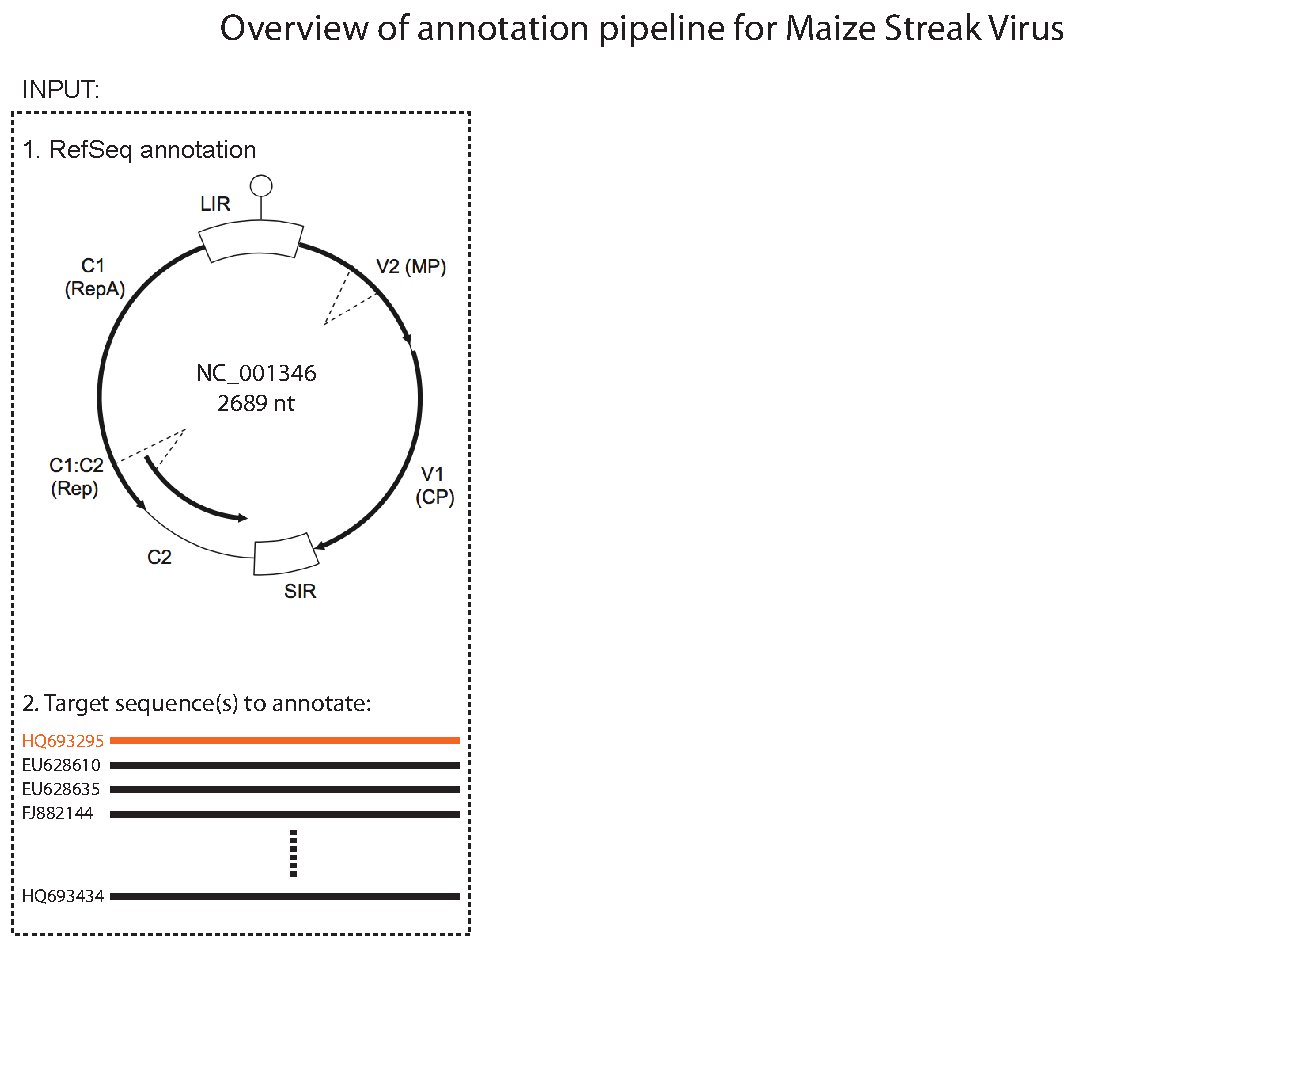
\includegraphics[width=10in]{figs/annotation-schematic-msv-1}
\end{center}
\vfill
\end{slide}
%%%%%%%%%%%%%%%%%%%%%%%%%%%%%%%%%%%%%%%%%%%%%%%%%%%%%%%%%%%%%%%%%%%%%%
\begin{slide}
\begin{center}
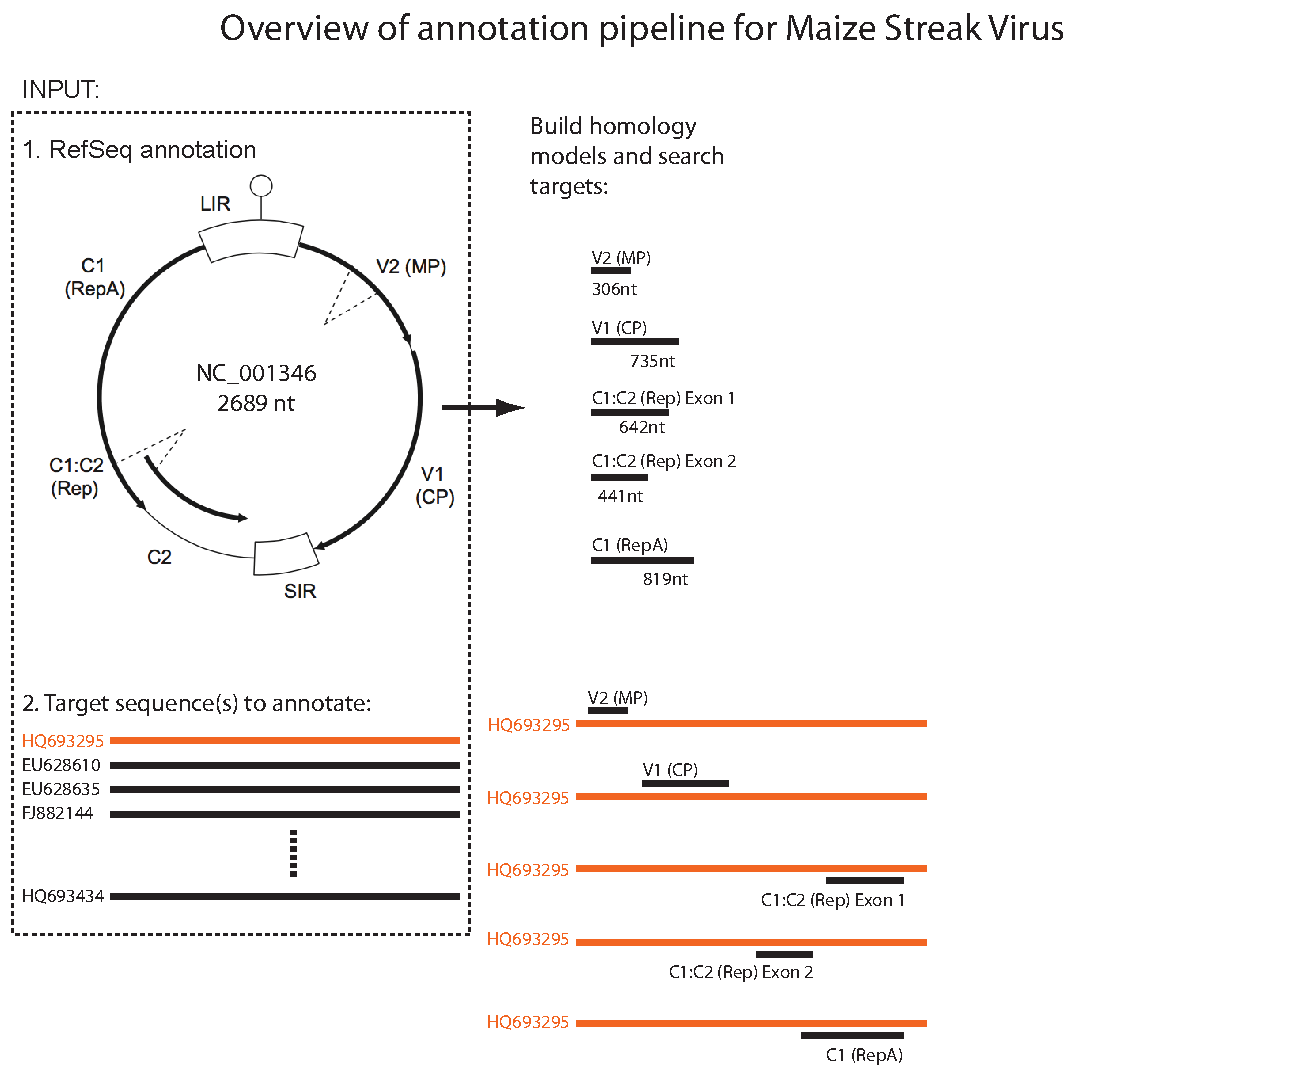
\includegraphics[width=10in]{figs/annotation-schematic-msv-2}
\end{center}
\vfill
\end{slide}
%%%%%%%%%%%%%%%%%%%%%%%%%%%%%%%%%%%%%%%%%%%%%%%%%%%%%%%%%%%%%%%%%%%%%%
\begin{slide}
\begin{center}
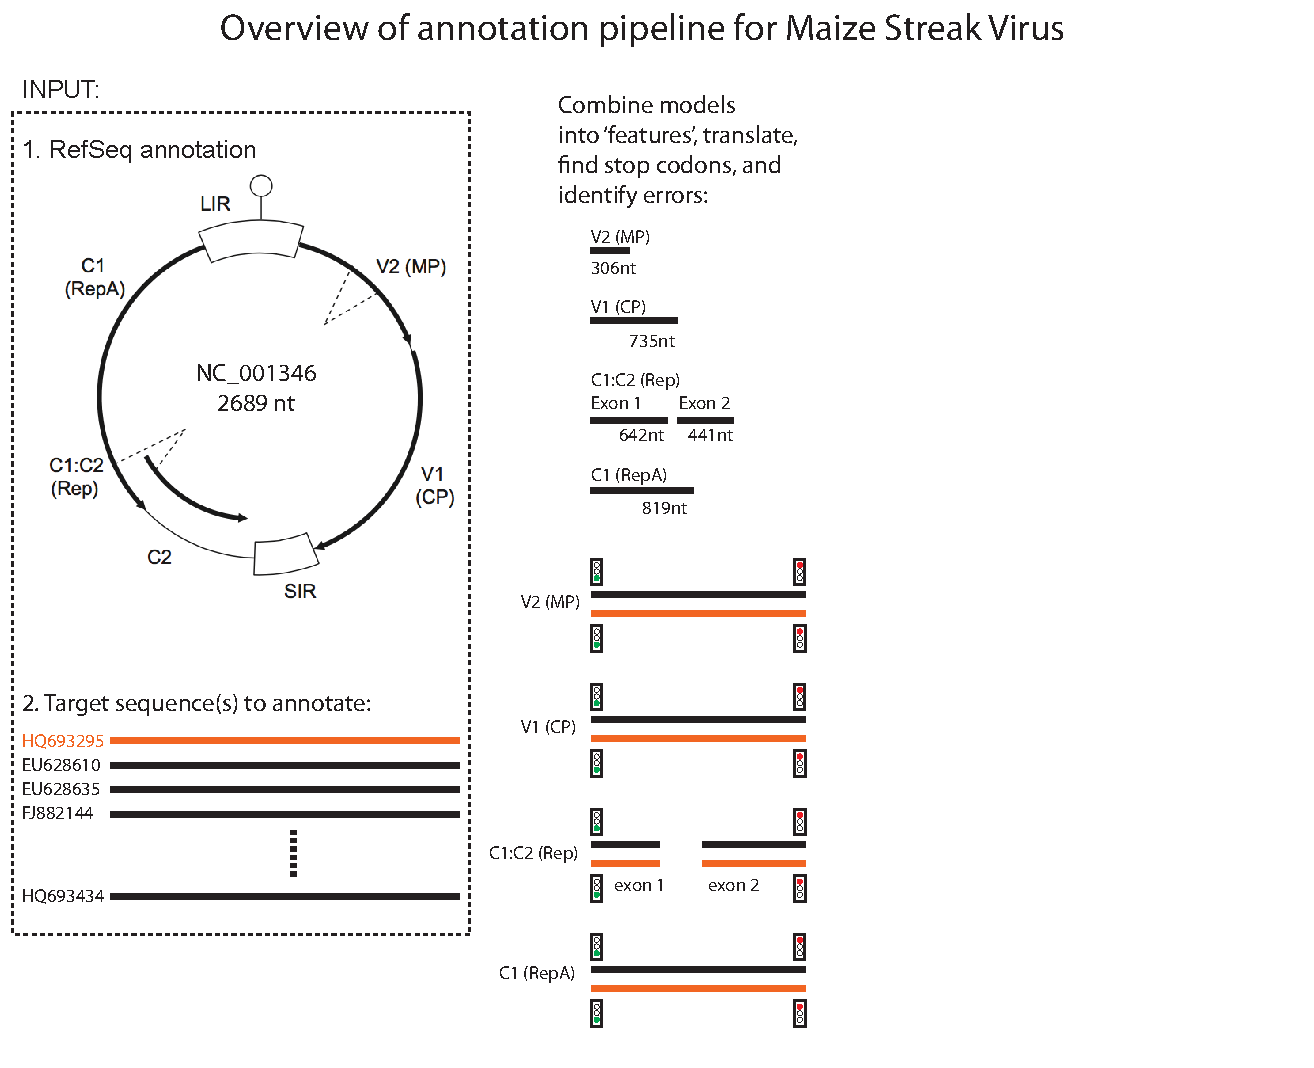
\includegraphics[width=10in]{figs/annotation-schematic-msv-3}
\end{center}
\vfill
\end{slide}
%%%%%%%%%%%%%%%%%%%%%%%%%%%%%%%%%%%%%%%%%%%%%%%%%%%%%%%%%%%%%%%%%%%%%%
\begin{slide}
\begin{center}
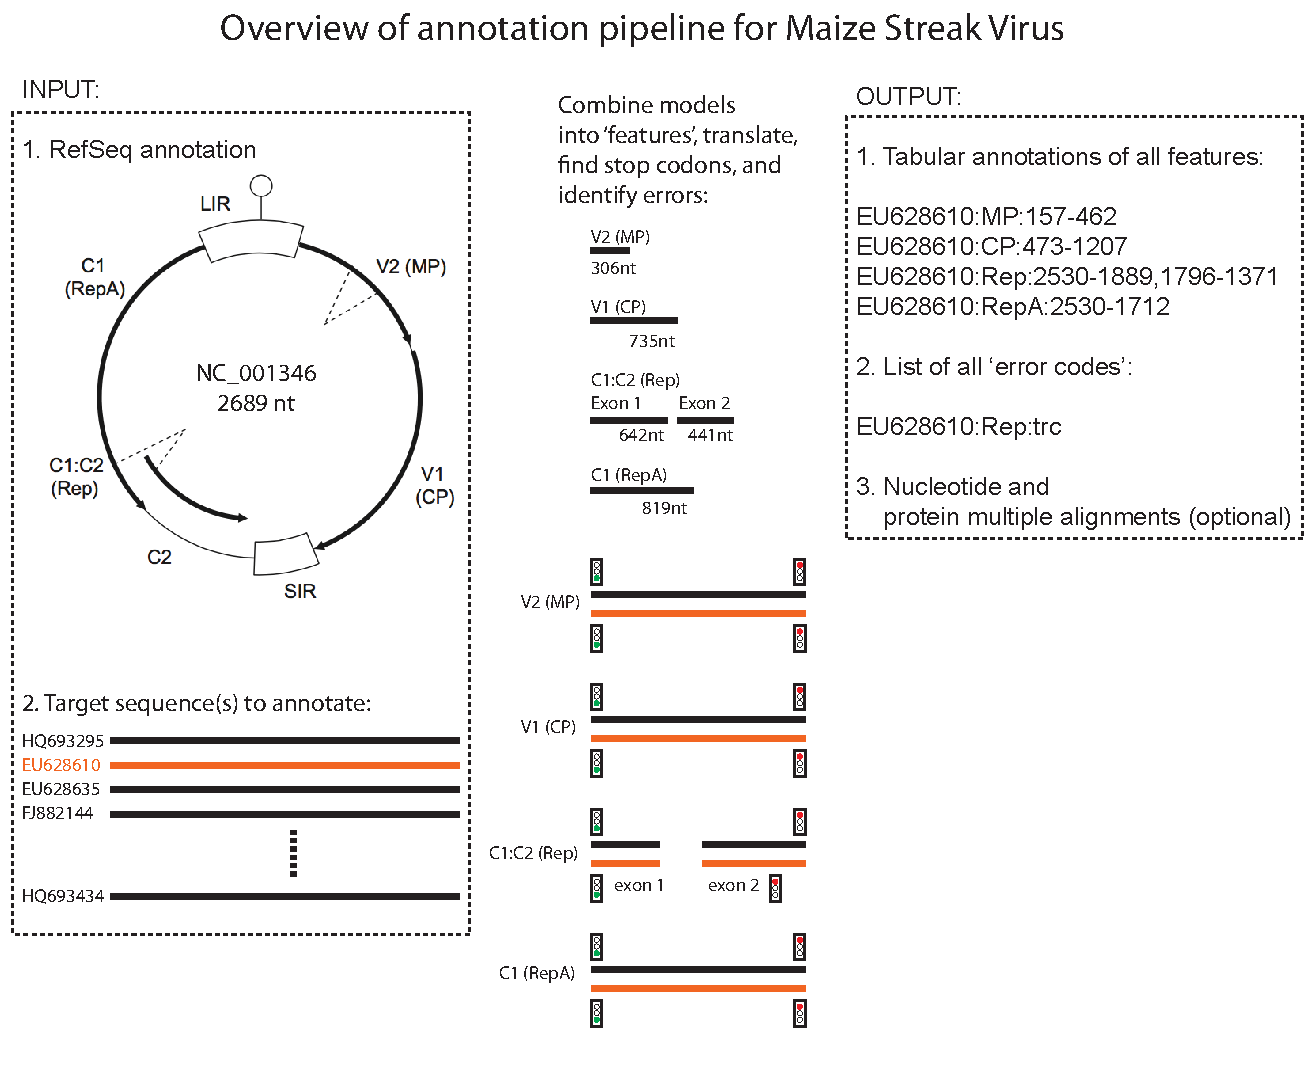
\includegraphics[width=10in]{figs/annotation-schematic-msv-4}
\end{center}
\vfill
\end{slide}
%%%%%%%%%%%%%%%%%%%%%%%%%%%%%%%%%%%%%%%%%%%%%%%%%%%%%%%%%%%%%%%%%%%%%%
\begin{slide}
\begin{center}
\includegraphics[width=10in]{figs/annotation-schematic-dengue-1}
\end{center}
\vfill
\end{slide}
%%%%%%%%%%%%%%%%%%%%%%%%%%%%%%%%%%%%%%%%%%%%%%%%%%%%%%%%%%%%%%%%%%%%%%
\begin{slide}
\begin{center}
\includegraphics[width=10in]{figs/annotation-schematic-dengue-2}
\end{center}
\vfill
\end{slide}
%%%%%%%%%%%%%%%%%%%%%%%%%%%%%%%%%%%%%%%%%%%%%%%%%%%%%%%%%%%%%%%%%%%%%%
\begin{slide}
\begin{center}
\includegraphics[width=10in]{figs/annotation-schematic-dengue-3}
\end{center}
\vfill
\end{slide}
%%%%%%%%%%%%%%%%%%%%%%%%%%%%%%%%%%%%%%%%%%%%%%%%%%%%%%%%%%%%%%%%%%%%%%
\begin{slide}
\begin{center}
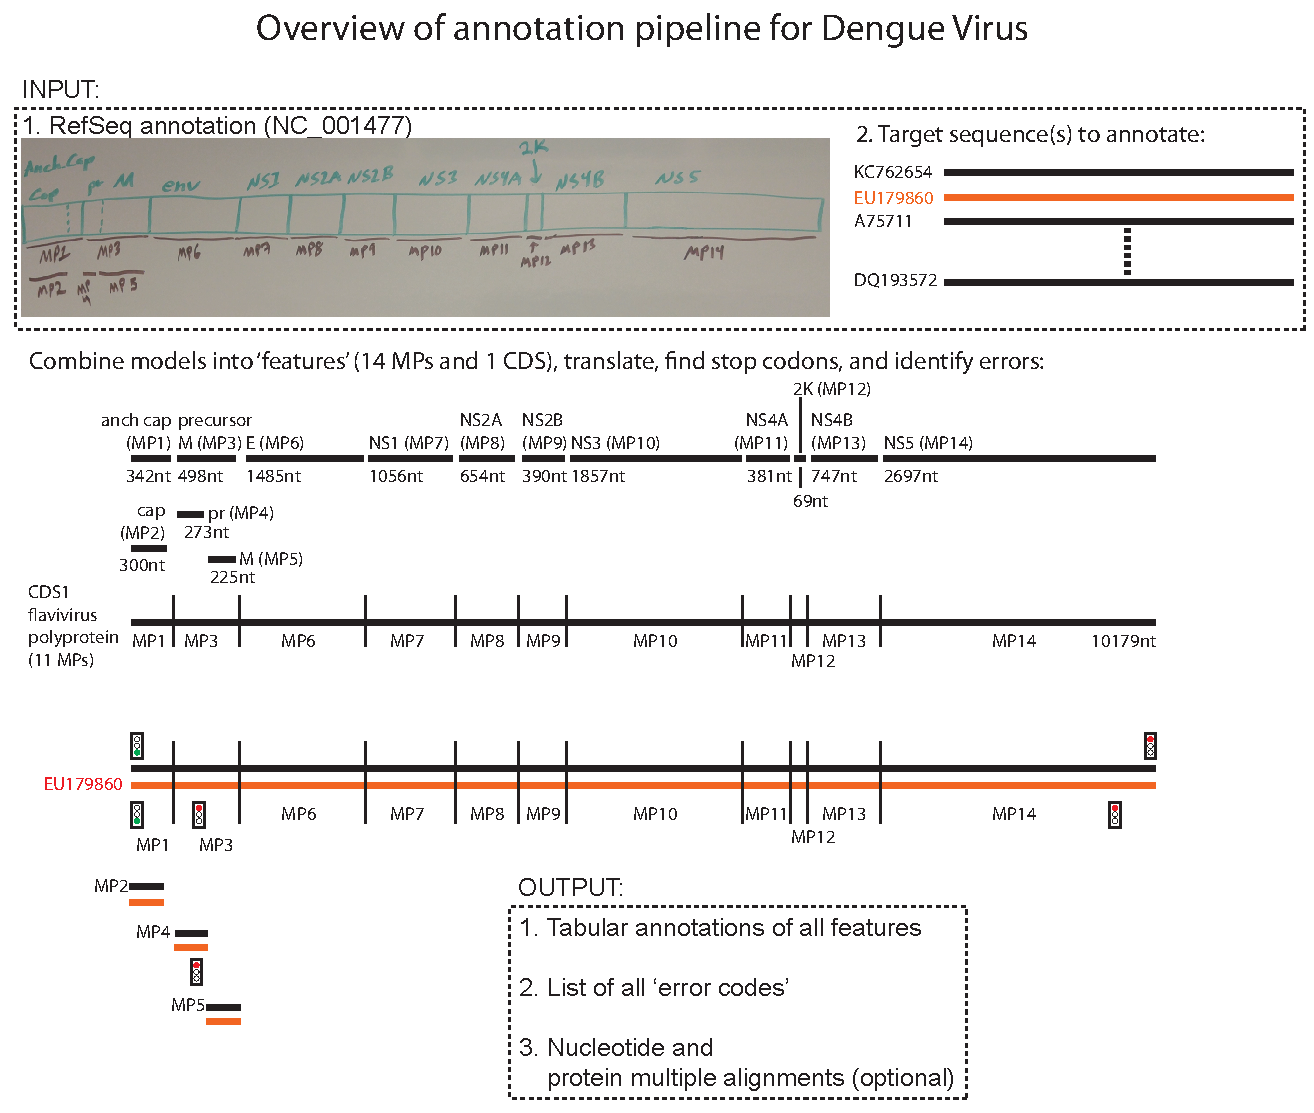
\includegraphics[width=10in]{figs/annotation-schematic-dengue-4-with-output}
\end{center}
\vfill
\end{slide}
%%%%%%%%%%%%%%%%%%%%%%%%%%%%%%%%%%%%%%%%%%%%%%%%%%%%%%%%%%%%%%%%%%%%%%
\begin{slide}
\begin{center}
\textbf{Error codes: 17 abnormal situations}

\small
\begin{itemize}
\item Per-feature (e.g. CDS, mature peptide) errors:
\begin{itemize}
\item Unexpected stop codon errors (trc, ext, nst, ntr)
\item Missing expected features (str, stp, nm3)
\item Problem with homology search prediction (bd5, bd3, nop)
\item Unexpected relationship to other features (olp, aja, ajb)
\item Problem annotating CDS due to mature peptide errors (aji, int, inp)
\end{itemize}
\item Per-sequence errors:
\begin{itemize} 
\item Lack of exactly one origin sequence (ori)
\end{itemize}
\end{itemize}

\end{center}
\vfill
\end{slide}
%%%%%%%%%%%%%%%%%%%%%%%%%%%%%%%%%%%%%%%%%%%%%%%%%%%%%%%%%%%%%%%%%%%%%%
\begin{slide}
\begin{center}
\textbf{trc error code reports a truncation due to an early stop codon}
\vspace{0.5in}

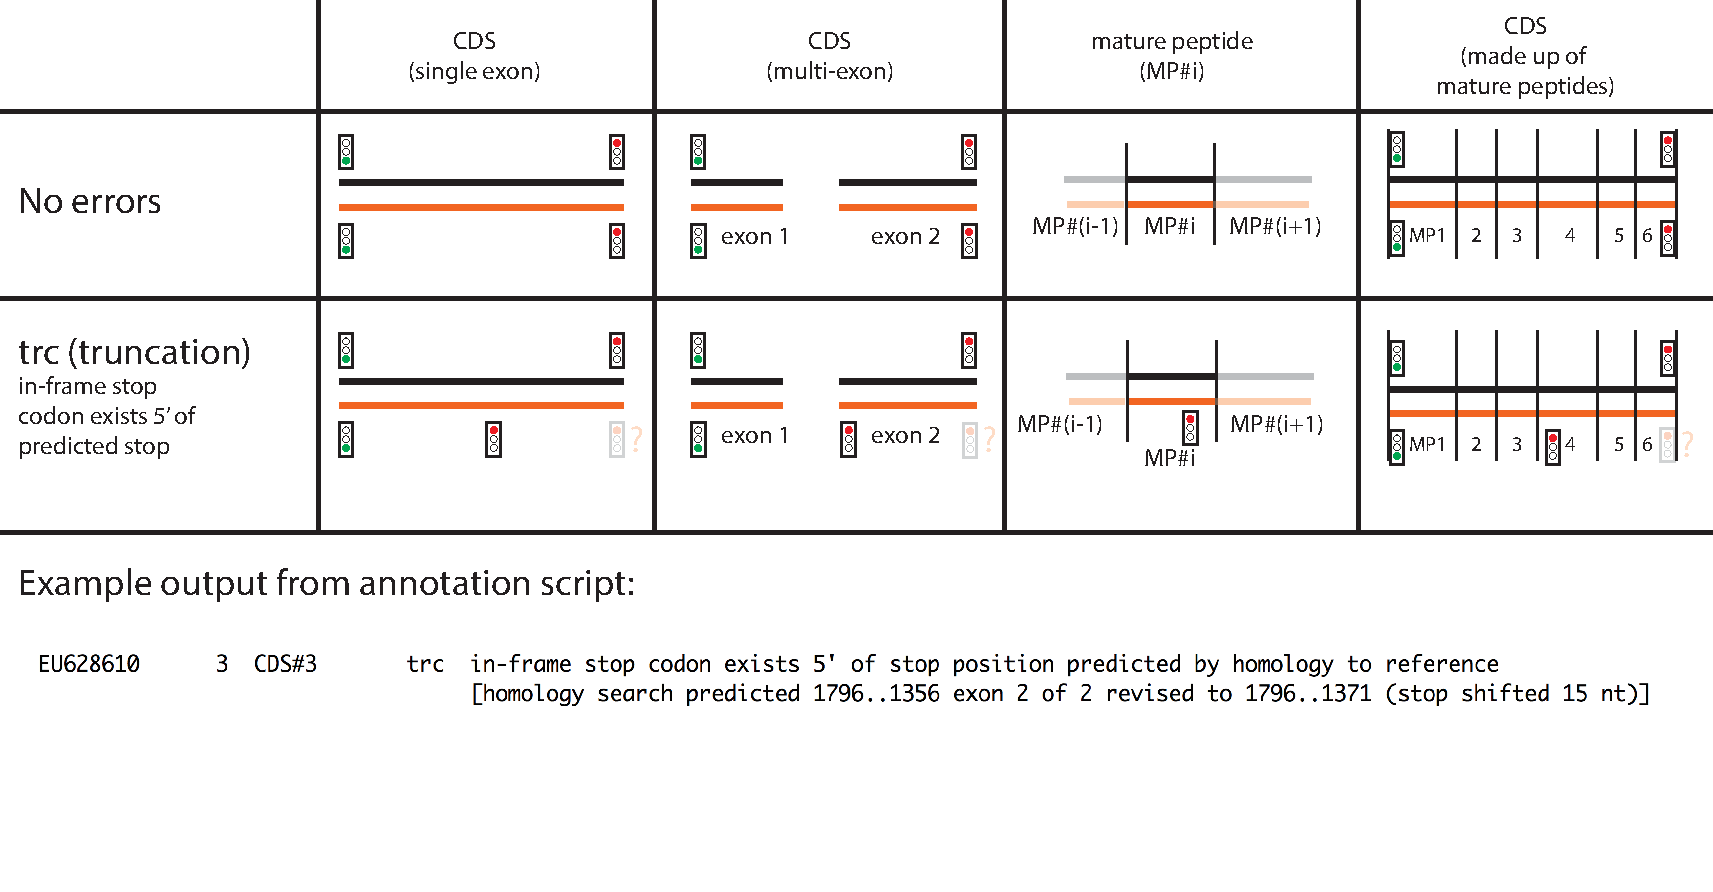
\includegraphics[width=10in]{figs/errornew-1-trc}
\end{center}
\vfill
\end{slide}
%%%%%%%%%%%%%%%%%%%%%%%%%%%%%%%%%%%%%%%%%%%%%%%%%%%%%%%%%%%%%%%%%%%%%%
\begin{slide}
\begin{center}
\textbf{ext: extended feature due to a missing stop codon}
\vspace{0.5in}

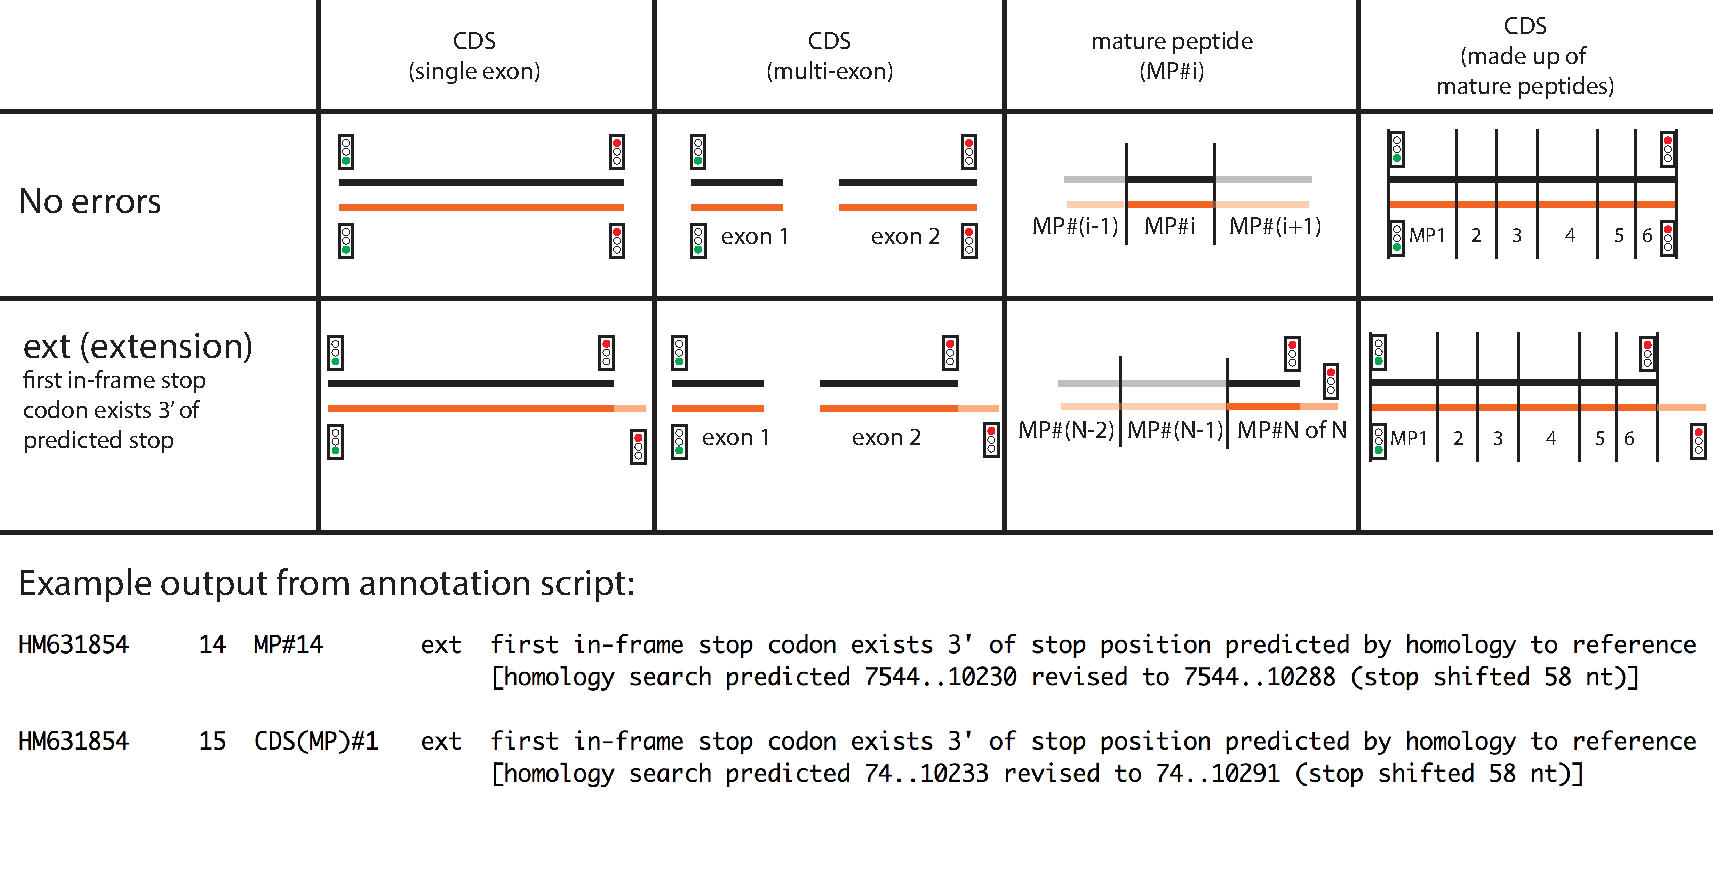
\includegraphics[width=10in]{figs/errornew-2-ext}
\end{center}
\vfill
\end{slide}
%%%%%%%%%%%%%%%%%%%%%%%%%%%%%%%%%%%%%%%%%%%%%%%%%%%%%%%%%%%%%%%%%%%%%%
\begin{slide}
\begin{center}
\textbf{olp: lack of an expected overlap with another feature}
\vspace{0.5in}

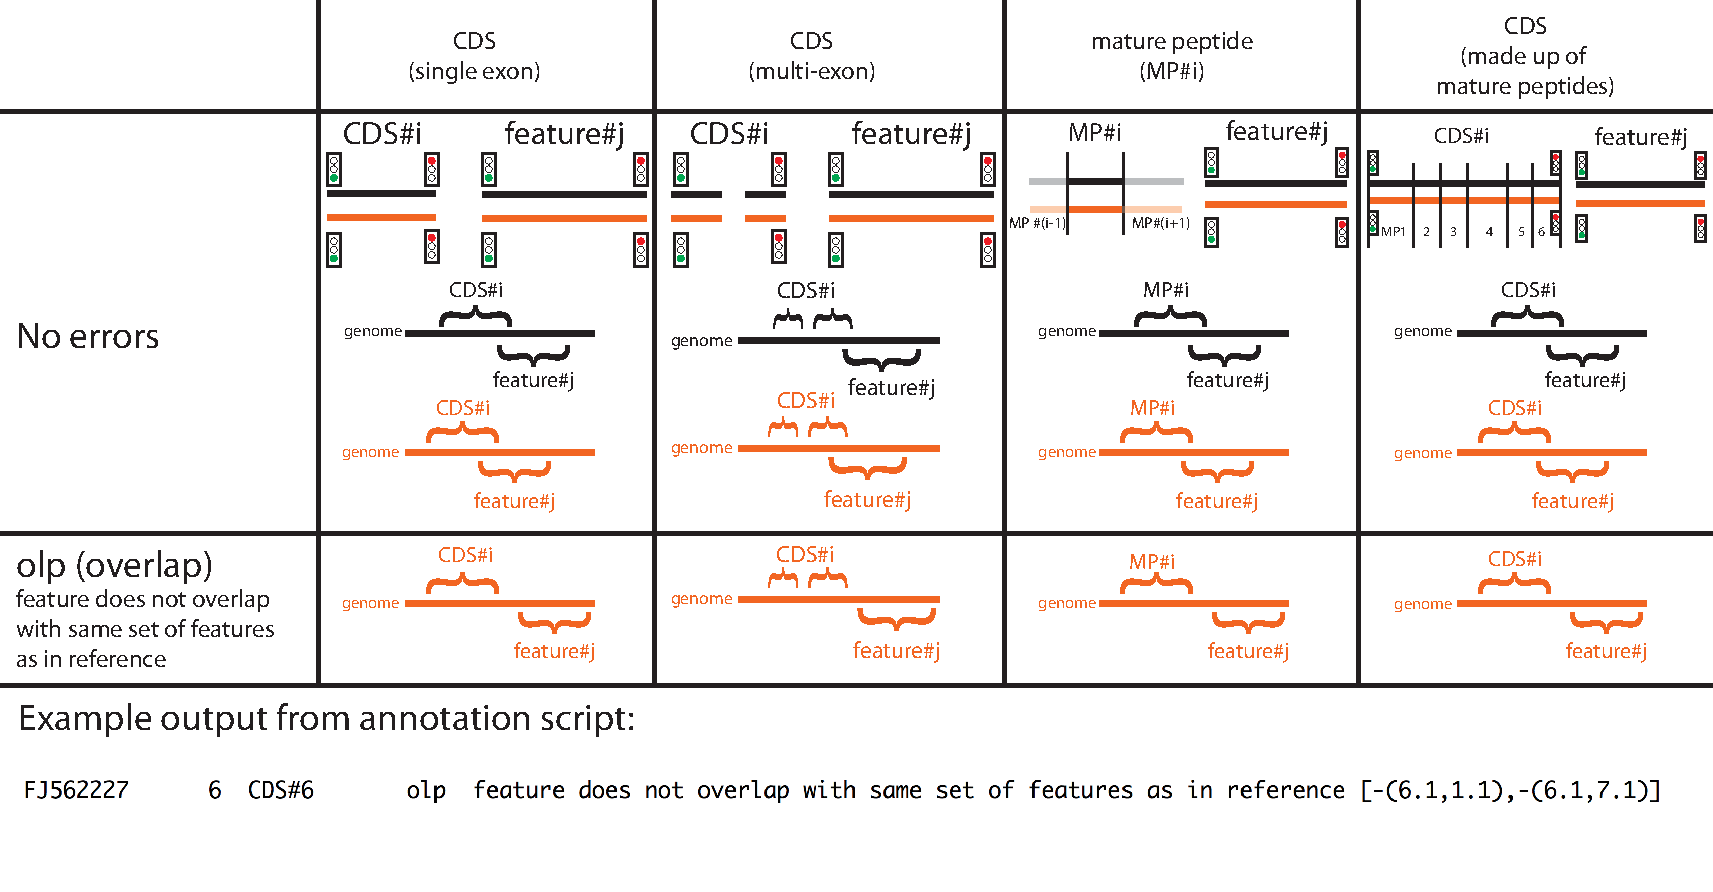
\includegraphics[width=10in]{figs/errornew-3-olp}
\end{center}
\vfill
\end{slide}
%%%%%%%%%%%%%%%%%%%%%%%%%%%%%%%%%%%%%%%%%%%%%%%%%%%%%%%%%%%%%%%%%%%%%%
\begin{slide}
\begin{center}
\textbf{ajb and aja error codes indicates lack of an expected adjacent feature}
\vspace{0.5in}

\includegraphics[width=10in]{figs/errornew-4-ajb}
\end{center}
\vfill
\end{slide}
%%%%%%%%%%%%%%%%%%%%%%%%%%%%%%%%%%%%%%%%%%%%%%%%%%%%%%%%%%%%%%%%%%%%%%
\begin{slide}
\begin{center}
\textbf{Outline of talk}

\small
\begin{description}
\item[1.] Selection of four pilot viral species
\item[2.] Overview of annotation pipeline and explanation of ``error codes''
\item[\textcolor{myorange}3.] \textcolor{myorange}{Statistics on pilot phase annotations}
\item[4.] Implementation of annotation pipeline
\item[5.] Interaction with J. Rodney Brister's Virus Variation group
\item[6.] Future directions
\end{description}

\end{center}
\vfill
\end{slide}
%%%%%%%%%%%%%%%%%%%%%%%%%%%%%%%%%%%%%%%%%%%%%%%%%%%%%%%%%%%%%%%%%%%%%%
\begin{slide}
\begin{center}
\textbf{Annotation statistics for pilot species \\ and comparison to
  GenBank annotations}

\includegraphics[height=7in]{figs/pilot-genbank-viv-comparison-table}
\vfill
\end{center}
\end{slide}
%%%%%%%%%%%%%%%%%%%%%%%%%%%%%%%%%%%%%%%%%%%%%%%%%%%%%%%%%%%%%%%%%%%%%%
\begin{slide}
\begin{center}
\includegraphics[height=8in]{figs/pilot-errcode-table-1}
\vfill
\end{center}
\end{slide}
%%%%%%%%%%%%%%%%%%%%%%%%%%%%%%%%%%%%%%%%%%%%%%%%%%%%%%%%%%%%%%%%%%%%%%
\begin{slide}
\begin{center}
\includegraphics[height=8in]{figs/pilot-errcode-table-2}
\vfill
\end{center}
\end{slide}
%%%%%%%%%%%%%%%%%%%%%%%%%%%%%%%%%%%%%%%%%%%%%%%%%%%%%%%%%%%%%%%%%%%%%%
\begin{slide}
\begin{center}
\includegraphics[height=8in]{figs/pilot-errcode-table-3}
\vfill
\end{center}
\end{slide}
%%%%%%%%%%%%%%%%%%%%%%%%%%%%%%%%%%%%%%%%%%%%%%%%%%%%%%%%%%%%%%%%%%%%%%
\begin{slide}
\begin{center}
\includegraphics[height=8in]{figs/pilot-errcode-table-4}
\vfill
\end{center}
\end{slide}
\begin{slide}
\begin{center}
\textbf{Outline of talk}

\small
\begin{description}
\item[1.] Selection of four pilot viral species
\item[2.] Overview of annotation pipeline and explanation of ``error codes''
\item[3.] Statistics on pilot phase annotations
\item[\textcolor{myorange}4.] \textcolor{myorange}{Implementation of annotation pipeline}
\item[4.] Interaction with J. Rodney Brister's Virus Variation group
\item[6.] Future directions
\end{description}

\end{center}
\vfill
\end{slide}
%%%%%%%%%%%%%%%%%%%%%%%%%%%%%%%%%%%%%%%%%%%%%%%%%%%%%%%%%%%%%%%%%%%%%%
\begin{slide}
\begin{center}
\includegraphics[width=10.5in]{figs/dnaorg-scripts-build1}
\vfill
\end{center}
\end{slide}
%%%%%%%%%%%%%%%%%%%%%%%%%%%%%%%%%%%%%%%%%%%%%%%%%%%%%%%%%%%%%%%%%%%%%%
\begin{slide}
\begin{center}
\includegraphics[width=10.5in]{figs/dnaorg-scripts-build2}
\vfill
\end{center}
\end{slide}
%%%%%%%%%%%%%%%%%%%%%%%%%%%%%%%%%%%%%%%%%%%%%%%%%%%%%%%%%%%%%%%%%%%%%%
\begin{slide}
\begin{center}
\includegraphics[width=10.5in]{figs/dnaorg-scripts-annotate1}
\vfill
\end{center}
\end{slide}
%%%%%%%%%%%%%%%%%%%%%%%%%%%%%%%%%%%%%%%%%%%%%%%%%%%%%%%%%%%%%%%%%%%%%%
\begin{slide}
\begin{center}
\includegraphics[width=10.5in]{figs/dnaorg-scripts-annotate2}
\vfill
\end{center}
\end{slide}
%%%%%%%%%%%%%%%%%%%%%%%%%%%%%%%%%%%%%%%%%%%%%%%%%%%%%%%%%%%%%%%%%%%%%%
\begin{slide}
\begin{center}
\includegraphics[width=10.5in]{figs/dnaorg-scripts-annotate3}
\vfill
\end{center}
\end{slide}
%%%%%%%%%%%%%%%%%%%%%%%%%%%%%%%%%%%%%%%%%%%%%%%%%%%%%%%%%%%%%%%%%%%%%%
\begin{slide}
\begin{center}
\includegraphics[width=10.5in]{figs/dnaorg-scripts-annotate4}
\vfill
\end{center}
\end{slide}
%%%%%%%%%%%%%%%%%%%%%%%%%%%%%%%%%%%%%%%%%%%%%%%%%%%%%%%%%%%%%%%%%%%%%%
\begin{slide}
\begin{center}
\textbf{Annotating Maize Streak Virus: dnaorg\_build.pl step} 

\includegraphics[width=10.5in]{figs/dnaorg-build-output}

\end{center}
\vfill
\end{slide}
%%%%%%%%%%%%%%%%%%%%%%%%%%%%%%%%%%%%%%%%%%%%%%%%%%%%%%%%%%%%%%%%%%%%%%
\begin{slide}
\begin{center}
\textbf{Annotating Maize Streak Virus: dnaorg\_annotate.pl step} 

\includegraphics[width=10.5in]{figs/dnaorg-annotate-output1}

\end{center}
\vfill
\end{slide}
%%%%%%%%%%%%%%%%%%%%%%%%%%%%%%%%%%%%%%%%%%%%%%%%%%%%%%%%%%%%%%%%%%%%%%
\begin{slide}
\begin{center}
\textbf{Annotating Maize Streak Virus: dnaorg\_annotate.pl step} 

\includegraphics[width=10.5in]{figs/dnaorg-annotate-output2}

\end{center}
\vfill
\end{slide}
%%%%%%%%%%%%%%%%%%%%%%%%%%%%%%%%%%%%%%%%%%%%%%%%%%%%%%%%%%%%%%%%%%%%%%
\begin{slide}
\begin{center}
\textbf{Infernal was chosen for homology search tool over HMMER 
  \\ because it encourages global alignment}

\begin{itemize}
\item HMMER3 alignments are local and often trim ends due to its
  probabilistic model

\center{\includegraphics[width=6in]{figs/hmmer-local-alignment}}\footnote{Eddy,
  PLoS Comput Biol 4.5 (2008): e1000069.}

\item Infernal encourages full length alignment by setting probability of
  global alignment to 0.5 (not shown). 
\end{itemize}

\vfill
\end{center}
\end{slide}
%%%%%%%%%%%%%%%%%%%%%%%%%%%%%%%%%%%%%%%%%%%%%%%%%%%%%%%%%%%%%%%%%%%%%%
\begin{slide}
\begin{center}
\textbf{Outline of talk}

\small
\begin{description}
\item[1.] Selection of four pilot viral species
\item[2.] Overview of annotation pipeline and explanation of ``error codes''
\item[3.] Statistics on pilot phase annotations
\item[4.] Implementation of annotation pipeline
\item[\textcolor{myorange}5.] \textcolor{myorange}{Interaction with J. Rodney Brister's Virus Variation group}
\item[6.] Future directions
\end{description}

\end{center}
\vfill
\end{slide}
%%%%%%%%%%%%%%%%%%%%%%%%%%%%%%%%%%%%%%%%%%%%%%%%%%%%%%%%%%%%%%%%%%%%%%
\begin{slide}
\begin{center}
\includegraphics[height=8in]{figs/eneida-slide-1}
\vfill
\end{center}
\end{slide}
%%%%%%%%%%%%%%%%%%%%%%%%%%%%%%%%%%%%%%%%%%%%%%%%%%%%%%%%%%%%%%%%%%%%%%
\begin{slide}
\begin{center}
\includegraphics[height=8in]{figs/eneida-slide-2}
\vfill
\end{center}
\end{slide}
%%%%%%%%%%%%%%%%%%%%%%%%%%%%%%%%%%%%%%%%%%%%%%%%%%%%%%%%%%%%%%%%%%%%%%
\begin{slide}
\begin{center}
\includegraphics[height=8in]{figs/eneida-slide-3}
\vfill
\end{center}
\end{slide}
%%%%%%%%%%%%%%%%%%%%%%%%%%%%%%%%%%%%%%%%%%%%%%%%%%%%%%%%%%%%%%%%%%%%%%
\begin{slide}
\begin{center}
\includegraphics[height=8in]{figs/eneida-slide-4}
\vfill
\end{center}
\end{slide}
%%%%%%%%%%%%%%%%%%%%%%%%%%%%%%%%%%%%%%%%%%%%%%%%%%%%%%%%%%%%%%%%%%%%%%
%%%%%%%%%%%%%%%%%%%%%%%%%%%%%%%%%%%%%%%%%%%%%%%%%%%%%%%%%%%%%%%%%%%%%%
\begin{slide}
\begin{center}
\textbf{Future directions}

\small
\begin{itemize}
\item Annotate more species (Norovirus, Zika, and Ebola are currently \\ being checked).

\item Long term:
\begin{itemize}
\item  Protein homology searches to supplement or replace nucleotide searches
\item  Given any viral sequence, find its nearest RefSeq
\item  Annotate structural RNA features (Infernal is well-suited for this)
\item  More robust solution to the problem of finding origin sequences
\item  Multiple alignment based homology searches 
\end{itemize}

\item Short term: we have a 36 item TODO list that we agreed to with
  J. Rodney \\ Brister's group on April 12, which includes:
\begin{itemize}
  \item Completed items (including analysis of West Nile annotations)
  \item Loading and using our pipeline's annotations in the Virus Variation
    database for Dengue and West Nile
  \item Reviewing Ebola and Norovirus annotations
  \item Comparing our Ebola annotations to existing annotations
\end{itemize}
\end{itemize}

\vfill
\end{center}
\end{slide}
%%%%%%%%%%%%%%%%%%%%%%%%%%%%%%%%%%%%%%%%%%%%%%%%%%%%%%%%%%%%%%%%%%%%%%
\begin{slide}

\large
\begin{center}
\large{\textbf{Acknowledgements}} \\

\vspace{0.5in}

Alejandro Sch\"{a}ffer \\
David Landsman \\
David Lipman

\vspace{0.5in}

J. Rodney Brister \\
Eneida Hatcher \\
Olga Blinkova \\
Sergey Zhdanov \\ 
Yiming Bao \\

\end{center}

\vfill
\end{slide}
%%%%%%%%%%%%%%%%%%%%%%%%%%%%%%%%%%%%%%%%%%%%%%%%%%%%%%%%%%%%%%%%%%%%%%
%%%%%%%%%%%%%%%%%%%%%%%%%%%%%%%%%%%%%%%%%%%%%%%%%%%%%%%%%%%%%%%%%%%%%%
\begin{slide}
\begin{center}
\textbf{Unexpected stop codon errors (trc,ntr)}
\vspace{0.5in}

\includegraphics[width=10in]{figs/error-1-trc-ntr}
\end{center}
\vfill
\end{slide}
%%%%%%%%%%%%%%%%%%%%%%%%%%%%%%%%%%%%%%%%%%%%%%%%%%%%%%%%%%%%%%%%%%%%%%
\begin{slide}
\begin{center}
\textbf{Unexpected stop codon errors (ext,nst)}
\vspace{0.5in}

\includegraphics[width=10in]{figs/error-2-ext-nst}
\end{center}
\vfill
\end{slide}
%%%%%%%%%%%%%%%%%%%%%%%%%%%%%%%%%%%%%%%%%%%%%%%%%%%%%%%%%%%%%%%%%%%%%%
\begin{slide}
\begin{center}
\textbf{Missing expected features (str,stp,nm3)}
\vspace{0.5in}

\includegraphics[width=10in]{figs/error-3-str-stp-nm3}
\end{center}
\vfill
\end{slide}
%%%%%%%%%%%%%%%%%%%%%%%%%%%%%%%%%%%%%%%%%%%%%%%%%%%%%%%%%%%%%%%%%%%%%%
\begin{slide}
\begin{center}
\textbf{Problem with homology search prediction (bd5,bd3,nop)}
\vspace{0.5in}

\includegraphics[width=10in]{figs/error-4-bd5-bd3-nop}
\end{center}
\vfill
\end{slide}
%%%%%%%%%%%%%%%%%%%%%%%%%%%%%%%%%%%%%%%%%%%%%%%%%%%%%%%%%%%%%%%%%%%%%%
\begin{slide}
\begin{center}
\textbf{Unexpected relationship to other features (olp)}
\vspace{0.5in}

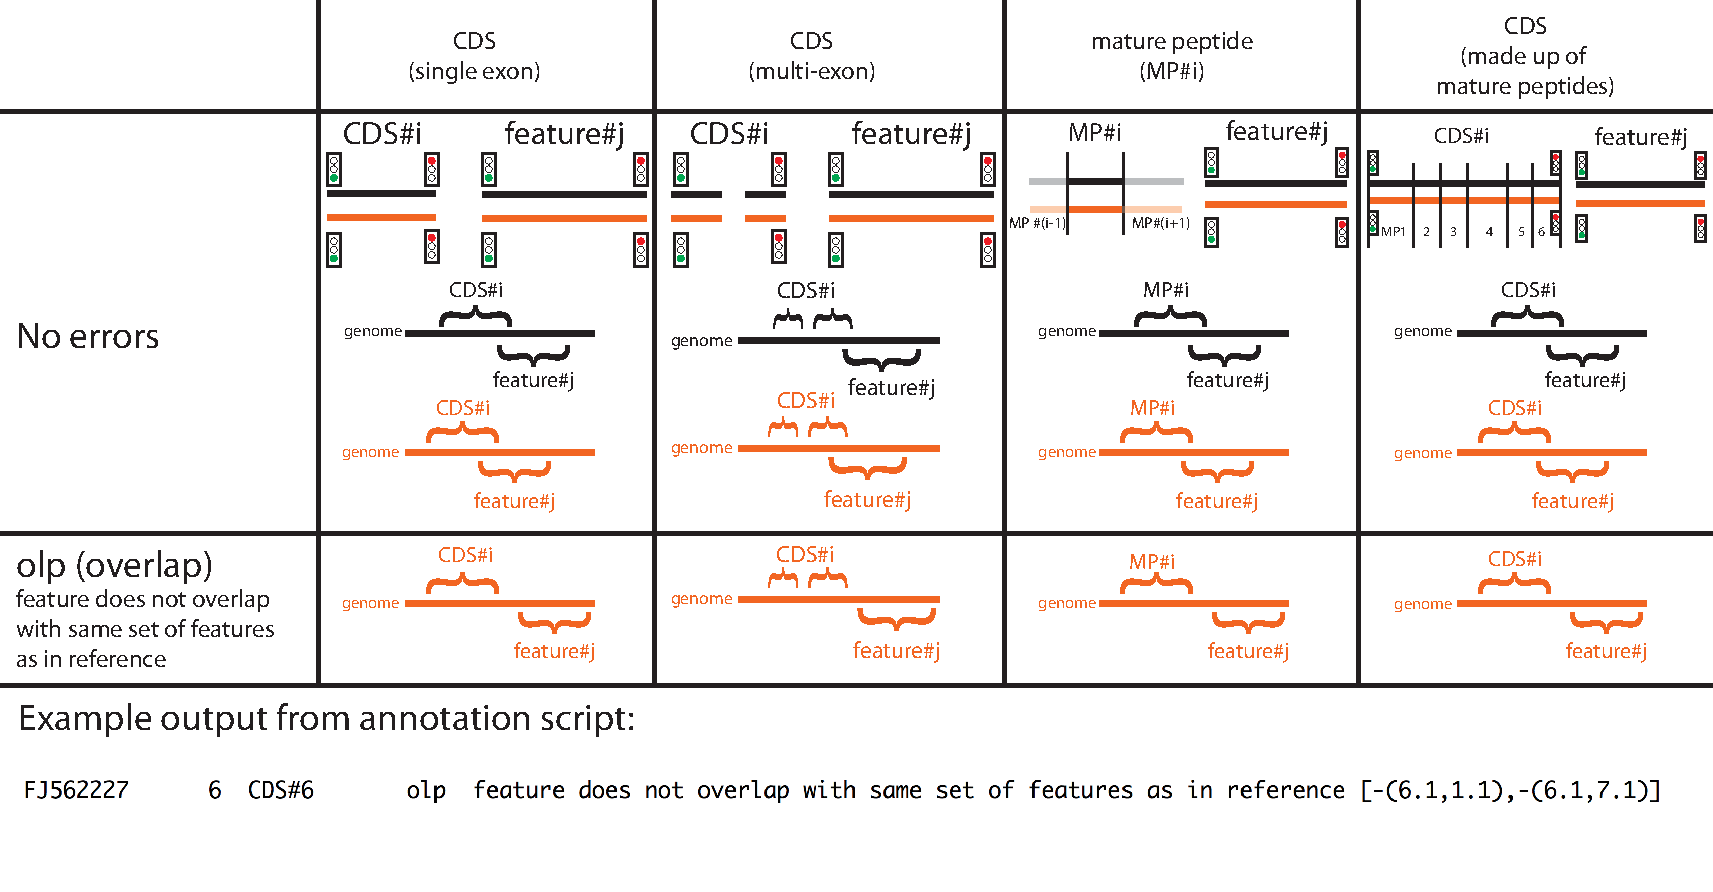
\includegraphics[width=10in]{figs/errornew-3-olp}
\end{center}
\vfill
\end{slide}
%%%%%%%%%%%%%%%%%%%%%%%%%%%%%%%%%%%%%%%%%%%%%%%%%%%%%%%%%%%%%%%%%%%%%%
\begin{slide}
\begin{center}
\textbf{Unexpected relationship to other features (ajb)}
\vspace{0.5in}

\includegraphics[width=10in]{figs/errornew-4-ajb}
\end{center}
\vfill
\end{slide}
%%%%%%%%%%%%%%%%%%%%%%%%%%%%%%%%%%%%%%%%%%%%%%%%%%%%%%%%%%%%%%%%%%%%%%
\begin{slide}
\begin{center}
\textbf{Unexpected relationship to other features (aja)}
\vspace{0.5in}

\includegraphics[width=10in]{figs/error-7-aja}
\end{center}
\vfill
\end{slide}
%%%%%%%%%%%%%%%%%%%%%%%%%%%%%%%%%%%%%%%%%%%%%%%%%%%%%%%%%%%%%%%%%%%%%%
\begin{slide}
\begin{center}
\textbf{Problem annotating CDS due to mature peptide errors (aji,int,inp)}
\vspace{0.5in}

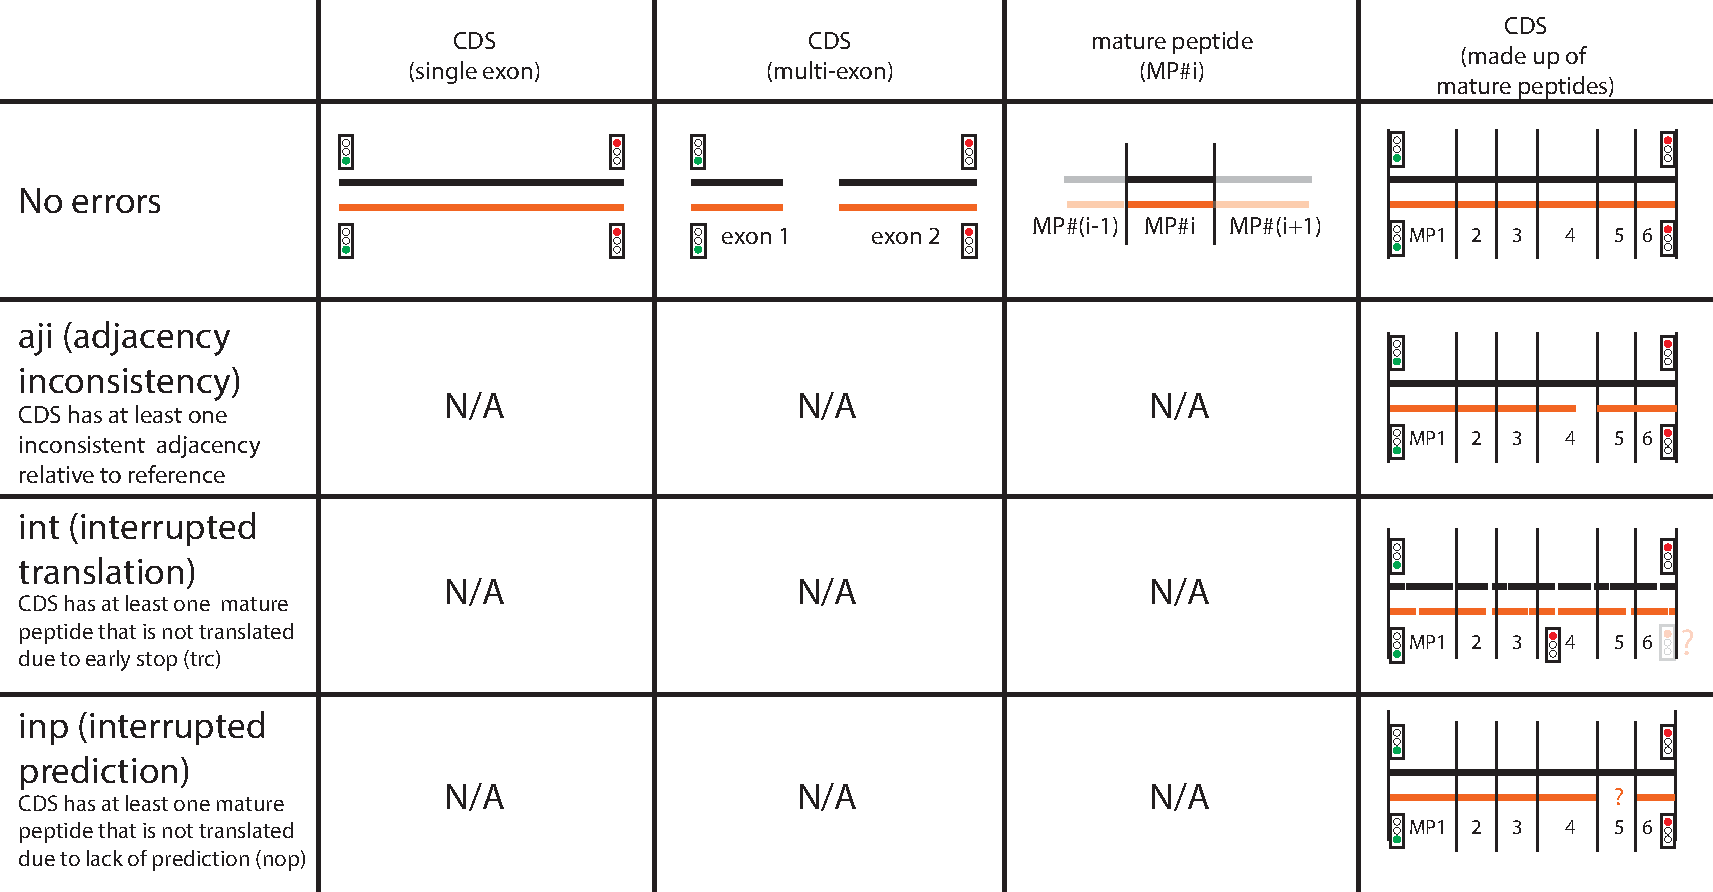
\includegraphics[width=10in]{figs/error-8-aji-int-inp}
\end{center}
\vfill
\end{slide}
%%%%%%%%%%%%%%%%%%%%%%%%%%%%%%%%%%%%%%%%%%%%%%%%%%%%%%%%%%%%%%%%%%%%%%
\begin{slide}
\begin{center}
\textbf{Lack of exactly one origin sequence (ori)}
\vspace{0.5in}

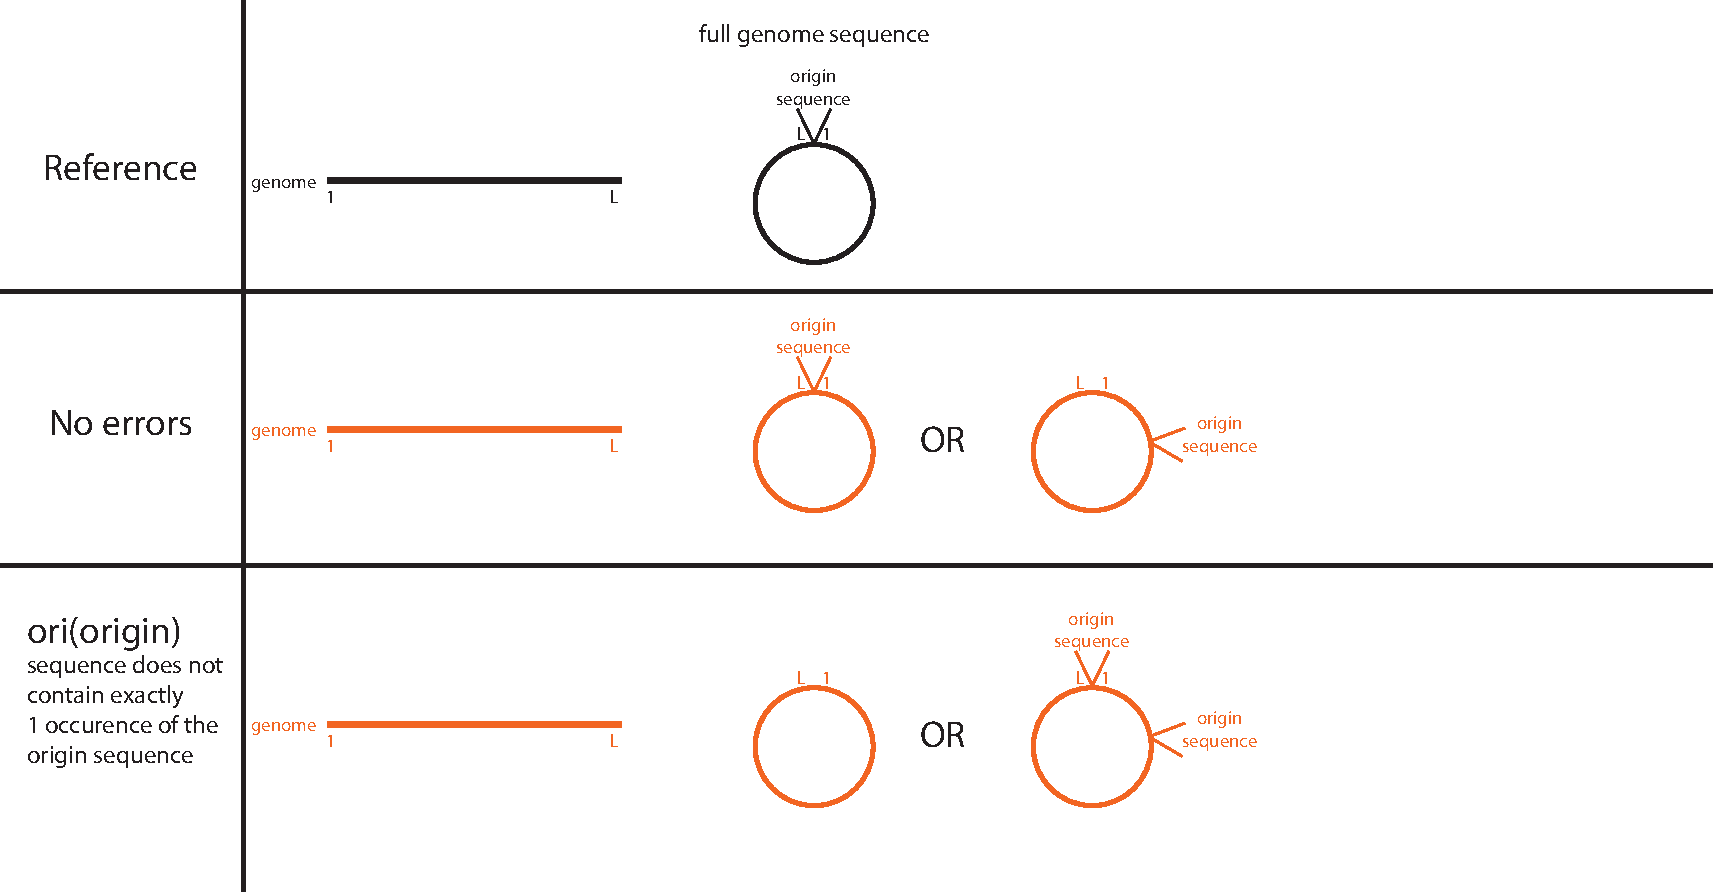
\includegraphics[width=10in]{figs/error-9-ori}
\end{center}
\vfill
\end{slide}
%%%%%%%%%%%%%%%%%%%%%%%%%%%%%%%%%%%%%%%%%%%%%%%%%%%%%%%%%%%%%%%%%%%%%%

\end{document}
